\begin{figure}
    \centering

    \newcommand{\nodescl}{0.7}
    \newcommand{\edgescl}{1}
    \newcommand{\wn}{\node[circle, draw, very thin, scale=\nodescl]}
\newcommand{\bn}{\node[circle, draw, very thin, scale=\nodescl, fill=black!25]}
\newcommand{\Wn}{\wn[ultra thick]}
\newcommand{\Bn}{\bn[ultra thick]}

\newcommand{\coordscl}[1] {#1*\edgescl}


    \begin{subfigure}[b]{0.25\textwidth}
        \centering

        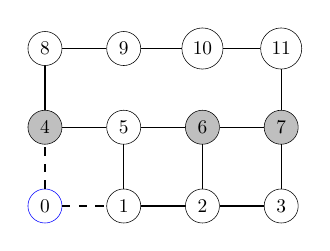
\begin{tikzpicture}
            \wn[draw=blue] (n0) at (\coordscl{0}, \coordscl{0}) {0};
            \wn (n1) at (\coordscl{1}, \coordscl{0}) {1};
            \wn (n2) at (\coordscl{2}, \coordscl{0}) {2};
            \wn (n3) at (\coordscl{3}, \coordscl{0}) {3};
            \bn (n4) at (\coordscl{0}, \coordscl{1}) {4};
            \wn (n5) at (\coordscl{1}, \coordscl{1}) {5};
            \bn (n6) at (\coordscl{2}, \coordscl{1}) {6};
            \bn (n7) at (\coordscl{3}, \coordscl{1}) {7};
            \wn (n8) at (\coordscl{0}, \coordscl{2}) {8};
            \wn (n9) at (\coordscl{1}, \coordscl{2}) {9};
            \wn (n10) at (\coordscl{2}, \coordscl{2}) {10};
            \wn (n11) at (\coordscl{3}, \coordscl{2}) {11};

            \draw[dashed]
                (n0) -- (n1)
                (n0) -- (n4)
                ;

            \draw
                (n1) -- (n2)
                (n2) -- (n3)
                (n2) -- (n6)
                (n6) -- (n5)
                (n7) -- (n6)
                (n4) -- (n8)
                (n11) -- (n7)
                (n8) -- (n9)
                (n9) -- (n10)
                (n10) -- (n11)
                (n1) -- (n5)
                (n3) -- (n7)
                (n4) -- (n5)
                ;
        \end{tikzpicture}
        
        
        \caption{Level-$i$ network}
        \label{fig:bmlrp-routes-all}
    \end{subfigure}%
    %
    \begin{subfigure}[b]{0.25\textwidth}
        \centering

        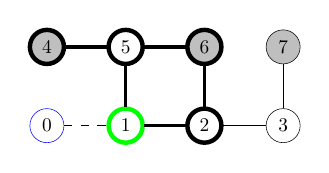
\begin{tikzpicture}
            \wn[draw=blue] (n0) at (\coordscl{0}, \coordscl{0}) {0};
            \Wn[draw=green] (n1) at (\coordscl{1}, \coordscl{0}) {1};
            \Wn (n2) at (\coordscl{2}, \coordscl{0}) {2};
            \wn (n3) at (\coordscl{3}, \coordscl{0}) {3};
            \Bn (n4) at (\coordscl{0}, \coordscl{1}) {4};
            \Wn (n5) at (\coordscl{1}, \coordscl{1}) {5};
            \Bn (n6) at (\coordscl{2}, \coordscl{1}) {6};
            \bn (n7) at (\coordscl{3}, \coordscl{1}) {7};
            
            \draw[dashed]
                (n0) -- (n1);

            \draw[very thick]
                (n1) -- (n2)
                (n4) -- (n5)
                (n1) -- (n5)
                (n2) -- (n6)
                (n5) -- (n6)
                ;

            \draw
                (n2) -- (n3)
                (n3) -- (n7)
                ;                
        \end{tikzpicture}

        \caption{Graph $G_0'$ of node 1}
        \label{fig:bmlrp-routes-nb1}
    \end{subfigure}%
    %
    \begin{subfigure}[b]{0.25\textwidth}
        \centering

        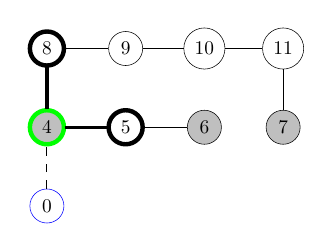
\begin{tikzpicture}
            \wn[draw=blue] (n0) at (\coordscl{0}, \coordscl{0}) {0};
            \Bn[draw=green] (n4) at (\coordscl{0}, \coordscl{1}) {4};
            \Wn (n5) at (\coordscl{1}, \coordscl{1}) {5};
            \bn (n6) at (\coordscl{2}, \coordscl{1}) {6};
            \bn (n7) at (\coordscl{3}, \coordscl{1}) {7};
            \Wn (n8) at (\coordscl{0}, \coordscl{2}) {8};
            \wn (n9) at (\coordscl{1}, \coordscl{2}) {9};
            \wn (n10) at (\coordscl{2}, \coordscl{2}) {10};
            \wn (n11) at (\coordscl{3}, \coordscl{2}) {11};

            \draw[dashed]
                (n0) -- (n4);

            \draw[very thick]
                (n4) -- (n5)
                (n4) -- (n8)
                ;

            \draw
                (n5) -- (n6)
                (n7) -- (n11)
                (n8) -- (n9)
                (n9) -- (n10)
                (n10) -- (n11)
                ;
        \end{tikzpicture}

        \caption{Graph $G_0'$ of node 4}
        \label{fig:bmlrp-routes-nb2}
    \end{subfigure}%
    %
    \begin{subfigure}[b]{0.25\textwidth}
        \centering

        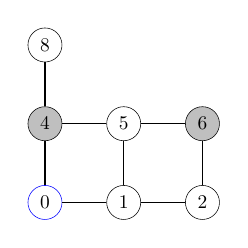
\begin{tikzpicture}
            \wn[draw=blue] (n0) at (\coordscl{0}, \coordscl{0}) {0};
            \wn (n1) at (\coordscl{1}, \coordscl{0}) {1};
            \wn (n2) at (\coordscl{2}, \coordscl{0}) {2};
            \bn (n4) at (\coordscl{0}, \coordscl{1}) {4};
            \wn (n5) at (\coordscl{1}, \coordscl{1}) {5};
            \bn (n6) at (\coordscl{2}, \coordscl{1}) {6};
            \wn (n8) at (\coordscl{0}, \coordscl{2}) {8};

            \draw
                (n0) -- (n1)
                (n1) -- (n2)
                (n0) -- (n4)
                (n1) -- (n5)
                (n2) -- (n6)
                (n4) -- (n5)
                (n5) -- (n6)
                (n4) -- (n8)
                ;
        \end{tikzpicture}

        \caption{Graph $G$ of node 0}
        \label{fig:bmlrp-routes-visible}
    \end{subfigure}%
    %

    \caption{Routes acquisition}
    \label{fig:bmlrp-routes}
\end{figure}
